\documentclass[../TST.tex]{subfiles}
\begin{document}
\begin{pproblem} A point mass oscillates harmonically along a line. The mass passes through a point $C$ of its trajectory in alternating time intervals of $\qty{1}{s}$, $\qty{2}{s}$, $\qty{1}{s}$, $\qty{2}{s}$, $\ldots$ . What is the ratio of the distances between $C$ and the endpoints of the trajectory?
\end{pproblem}
\ifprob \else
	\begin{solution} Let the motion have an amplitude $A$ and angular frequency $\omega$. Without loss of generality, we can describe it with $x=A\cos{(\omega t)}$. Let the position of point $C$ be $x_0$. We want to find $x_0/A$. A clean way to do this is to note that $x$ can be interpreted as the projection along the $x$-axis of a vector with magnitude $A$ which rotates counterclockwise with an angular frequency $\omega$:
		\begin{center}
		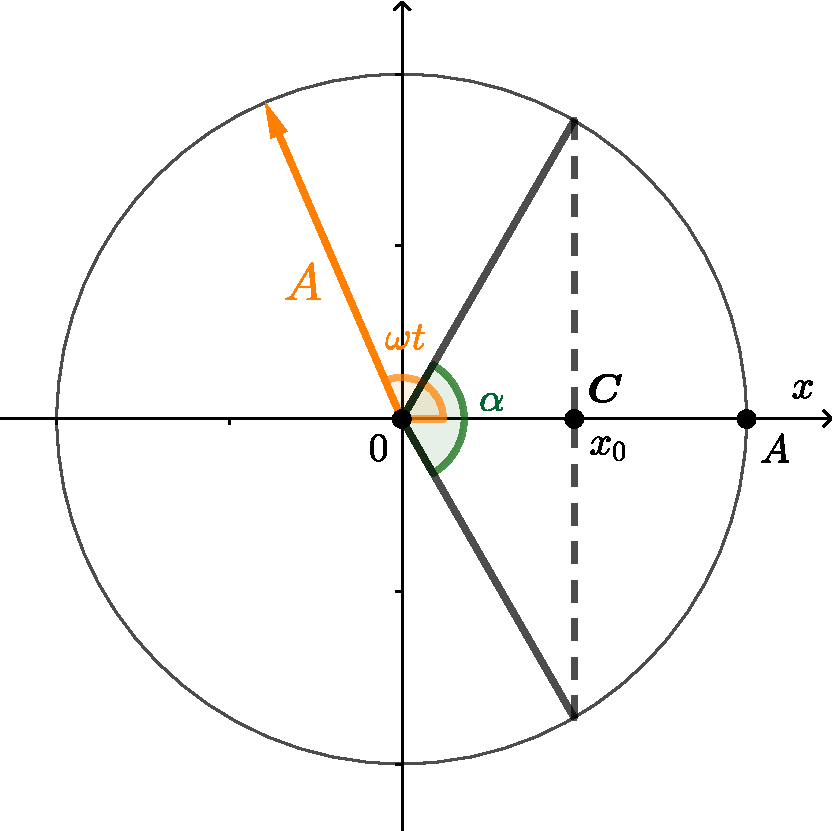
\includegraphics[width=0.4\textwidth]{fig/a2012_s1.pdf}
		\end{center}
Between two consecutive crossings of $C$ the vector rotates either by $\alpha$ or $2\pi - \alpha$. Assuming $\alpha <\pi$, we know that
\begin{equation*}
\frac{\alpha}{2\pi-\alpha}=\frac{\qty{1}{s}}{\qty{2}{s}}
.
\end{equation*}
Then $\alpha = \frac{2\pi}{3}$. On the other hand, $\cos{\frac{\alpha}{2}}=\frac{x_0}{A}$, so $\frac{x_0}{A}=\frac{1}{2}$. The distances between $C$ and the endpoints are $A-x_0$ and $A+x_0$, so the ratio is
\begin{equation*}
	q=\frac{A-x_0}{A+x_0}=\frac{1-({x_0}/{A})}{1+({x_0}/{A})}=\boxed{\frac{1}{3}.}
\end{equation*}

\end{solution}
\fi
\end{document}
